
%{{第五十九回}}{第五十九回}}

\chapter{柳叶渚边嗔莺咤燕\hspace{.5em}绛芸轩里召将飞符}

{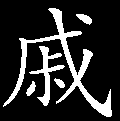
\includegraphics[width=3mm]{../Images/00005}山无起伏,便是顽山;水无潆洄,便是死水。此回于前回叙过事,字字应;于后回未叙事,语语伏。是上下关节。至铸鼎象物手段,则在下回施展。}

话说宝玉听说贾母等回来,随多添了一件衣服,拄杖前边来,都见过了。贾母等因每日辛苦,都要早些歇息,一宿无话,次日五鼓,又往朝中去。

离送灵日不远,鸳鸯、琥珀、翡翠、玻璃四人都忙着打点贾母之物,玉钏、彩云、彩霞等皆打叠王夫人之物,当面查点与跟随的管事媳妇们。跟随的一共大小六个丫鬟,十个老婆子媳妇子,男人不算。连日收拾驮轿器械。鸳鸯与玉钏儿皆不随去,只看屋子。一面先几日预发帐幔铺陈之物,先有四五个媳妇并几个男人领了出来,坐了几辆车绕道先至下处,铺陈安插等候。

临日,贾母带着蓉妻坐一乘驮轿,王夫人在后亦坐一乘驮轿,贾珍骑马率了众家丁护卫。又有几辆大车与婆子丫鬟等坐,并放些随换的衣包等件。是日薛姨妈尤氏率领诸人直送至大门外方回。贾琏恐路上不便,一面打发了他父母起身赶上贾母王夫人驮轿,自己也随后带领家丁押后跟来。

荣府内赖大添派人丁上夜,将两处厅院都关了,一应出入人等皆走西边小角门。日落时,便命关了仪门,不放人出入。园中前后东西角门亦皆关锁,只留王夫人大房之后常系他姊妹出入之门、东边通薛姨妈的角门,这两门因在内院,不必关锁。里面鸳鸯和玉钏儿也各将上房关了,自领丫鬟婆子下房去安歇。每日林之孝之妻进来,带领十来个婆子上夜,穿堂内又添了许多小厮们坐更打梆子,已安插得十分妥当。

一日清晓,宝钗春困已醒,搴帷下榻,微觉轻寒,启户视之,见园中土润苔青,原来五更时落了几点微雨。于是唤起湘云等人来,一面梳洗,湘云因说两腮作痒,恐又犯了杏癍癣,因问宝钗要些蔷薇硝来。宝钗道:``前儿剩的都给了妹子。''因说:``颦儿配了许多,我正要和他要些,因今年竟没发痒,就忘了。''因命莺儿去取些来。莺儿应了才去时,蕊官便说:``我同你去,顺便瞧瞧藕官。''说着,一径同莺儿出了蘅芜苑。

二人你言我语,一面行走,一面说笑,不觉到了柳叶渚\href{../Text/part0063_split_000.html\#lnkback_1_a}{\textsuperscript{①}},顺着柳堤走来。因见柳叶才吐浅碧,丝若垂金,莺儿便笑道:``你会拿着柳条子编东西不会?''蕊官笑道:``编什么东西?''莺儿道:``什么编不得?顽的使的都可。等我摘些下来,带着这叶子编个花篮儿,采了各色花放在里头,才是好顽呢。''说着,且不去取硝,且伸手挽翠披金,采了许多的嫩条,命蕊官拿着。他却一行走一行编花篮,随路见花便采一二枝,编出一个玲珑过梁的篮子。枝上自有本来翠叶满布,将花放上,却也别致有趣。喜的蕊官笑道:``姐姐,给了我罢。''莺儿道:``这一个咱们送林姑娘,回来咱们再多采些,编几个大家顽。''说着,来至潇湘馆中。

黛玉也正晨妆,见了篮子,便笑说:``这个新鲜花篮是谁编的?''莺儿笑说:``我编了送姑娘顽的。''黛玉接了笑道:``怪道人赞你的手巧,这顽意儿却也别致。''一面瞧了,一面便命紫鹃挂在那里。莺儿又问候了薛姨妈,方和黛玉要硝。黛玉忙命紫鹃包了一包,递与莺儿。黛玉又道:``我好了,今日要出去逛逛。你回去说与姐姐,不用过来问候妈了,也不敢劳他来瞧我,梳了头同妈都往你那里去,连饭也端了那里去吃,大家热闹些。''

莺儿答应了出来,便到紫鹃房中找蕊官。只见藕官与蕊官二人正说得高兴,不能相舍,因说:``姑娘也去呢,藕官先同我们去等着岂不好?''紫鹃听如此说,便也说道:``这话倒是,他这里淘气的也可厌。''一面说,一面便将黛玉的匙箸用一块洋巾包了,交与藕官道:``你先带了这个去,也算一趟差了。''藕官接了,笑嘻嘻同他二人出来,一径顺着柳堤走来。莺儿便又采些柳条,越性坐在山石上编起来,又命蕊官先送了硝去再来。他二人只顾爱看他编,那里舍得去。莺儿只顾催说:``你们再不去,我也不编了。''藕官便说:``我同你去了再快回来。''二人方去了。

这里莺儿正编,只见何婆的女儿春燕走来,笑问:``姐姐编什么呢?''正说着,蕊、藕二人也到了。春燕便向藕官道:``前儿你到底烧什么纸?被我姨妈看见了,要告你没告成,倒被宝玉赖了他一大些不是,气的他一五一十告诉我妈。你们在外头这二三年积了些什么仇恨,如今还不解开?''藕官冷笑道:``有什么仇恨?他们不知足,反怨我们了。在外头这两年,别的东西不算,只算我们的米菜,不知赚了多少家去,合家子吃不了,还有每日买东买西赚的钱。在外逢我们使他们一使儿,就怨天怨地的。你说说可有良心?''春燕笑道:``他是我的姨妈,也不好向着外人反说他的。怨不得宝玉说:`女孩儿未出嫁,是颗无价之宝珠;出了嫁,不知怎么就变出许多的不好的毛病\href{../Text/part0063_split_000.html\#lnkback_2_a}{\textsuperscript{②}}来,虽是颗珠子,却没有光彩宝色,是颗死珠了;再老了,更变的不是珠子,竟是鱼眼睛了。分明一个人,怎么变出三样来?'这话虽是混话,倒也有些不差。别人不知道,只说我妈和姨妈,他老姊妹两个,如今越老了越把钱看的真了。先时老姐儿两个在家抱怨没个差使,没个进益,幸亏有了这园子,把我挑进来,可巧把我分到怡红院。家里省了我一个人的费用不算外,每月还有四五百钱的馀剩,这也还说不够。后来老姊妹二人都派到梨香院去照看他们,藕官认了我姨妈,芳官认了我妈,这几年着实宽裕了。如今挪进来也算撒开手了,还只无厌。你说好笑不好笑?我姨妈刚和藕官吵了,接着我妈为洗头就和芳官吵。芳官连要洗头也不给他洗。昨日得月钱,推不去了,买了东西先叫我洗。我想了一想:我自有钱,就没钱要洗时,不管袭人、晴雯、麝月,那一个跟前和他们说一声,也都容易,何必借这个光儿?好没意思。所以我不洗。他又叫我妹妹小鸠儿洗了,才叫芳官,果然就吵起来。接着又要给宝玉吹汤,你说可笑死了人?我见他一进来,我就告诉那些规矩。他只不信,只要强做知道的,足的讨个没趣儿。幸亏园里的人多,没人分记的清楚谁是谁的亲故。若有人记得,只有我们一家人吵,什么意思呢?你这会子又跑了来弄这个。这一带地上的东西都是我姑娘管着,一得了这地方,比得了永远基业还利害,每日早起晚睡,自己辛苦了还不算,每日逼着我们来照看,生恐有人糟踏,又怕误了我的差使。如今进来了,老姑嫂两个照看得谨谨慎慎,一根草也不许人动。你还掐这些花儿,又折他的嫩树,他们即刻就来,仔细他们抱怨。''莺儿道:``别人乱折乱掐使不得,独我使得。自从分了地基之后,每日里各房皆有分例,吃的不用算,单管花草顽意儿。谁管什么,每日谁就把各房里姑娘丫头戴的,必要各色送些折枝的去,还有插瓶的。惟有我们说了:`一概不用送,等要什么再和你们要。'究竟没有要过一次。我今便掐些,他们也不好意思说的。''

一语未了,他姑娘果然拄了拐走来。莺儿春燕等忙让坐。那婆子见采了许多嫩柳,又见藕官等都采了许多鲜花,心内便不受用;看着莺儿编,又不好说什么,便说春燕道:``我叫你来照看照看,你就贪住顽不去了。倘或叫起你来,你又说我使你了,拿我做隐身符儿你来乐。''春燕道:``你老又使我,又怕,这会子反说我。难道把我劈做八瓣子不成?''莺儿笑道:``姑妈,你别信小燕的话。这都是他摘下来的,烦我给他编,我撵他,他不去。''春燕笑道:``你可少顽儿。你只顾顽儿,他老人家就认真了。''那婆子本是愚顽之辈,兼之年近昏耄,惟利是命,一概情面不管,正心疼肝断,无计可施,听莺儿如此说,便以老卖老,拿起拄杖来向春燕身上击上几下,骂道:``小蹄子,我说着你,你还和我强嘴儿呢。你妈恨的牙根痒痒,要撕你的肉吃呢。你还来和我强梆子似的。''打的春燕又愧又急,哭道:``莺儿姐姐顽话,你老就认真打我。我妈为什么恨我?我又没烧胡了洗脸水,有什么不是!''莺儿本是顽话,忽见婆子认真动了气,忙上去拉住,笑道:``我才是顽话,你老人家打他,我岂不愧?''那婆子道:``姑娘,你别管我们的事,难道为姑娘在这里,不许我管孩子不成?''莺儿听见这般蠢话,便赌气红了脸,撒了手冷笑道:``你老人家要管,那一刻管不得,偏我说了一句顽话就管他了。我看你老管去!''说着,便坐下,仍编柳篮子。

偏又有春燕的娘出来找他,喊道:``你不来舀水,在那里做什么呢?''那婆子便接声儿道:``你来瞧瞧,你的女儿连我也不服了!在那里排揎我呢。''那婆子一面走过来说:``姑奶奶,又怎么了?我们丫头眼里没娘罢了,连姑妈也没了不成?''莺儿见他娘来了,只得又说原故。他姑娘那里容人说话,便将石上的花柳与他娘瞧道:``你瞧瞧,你女儿这么大孩子顽的。他先领着人糟踏我,我怎么说人?''他娘也正为芳官之气未平,又恨春燕不遂他的心,便走上来打耳刮子,骂道:``小娼妇,你能上去了几年?你也跟那起轻狂浪小妇学,怎么就管不得你们了?干的我管不得,你是我屄里掉出来的,难道也不敢管你不成!既是你们这起蹄子到的去的地方我到不去,你就该死在那里伺候,又跑出来浪汉。''一面又抓起柳条子来,直送到他脸上,问道:``这叫作什么?这编的是你娘的屄!''莺儿忙道:``那是我们编的,你老别指桑骂槐。''那婆子深妒袭人晴雯一干人,已知凡房中大些的丫鬟都比他们有些体统权势,凡见了这一干人,心中又畏又让,未免又气又恨,亦且迁怒于众,复又看见了藕官,又是他令姊的冤家,四处凑成一股怒气。

那春燕啼哭着往怡红院去了。他娘又恐问他为何哭,怕他又说出自己打他,又要受晴雯等之气,不免着起急来,又忙喊道:``你回来!我告诉你再去。''春燕那里肯回来?急的他娘跑了去又拉他。他回头看见,便也往前飞跑。他娘只顾赶他,不防脚下被青苔滑倒,引的莺儿三个人反都笑了。莺儿便赌气将花柳皆掷于河中,自回房去。这里把个婆子心疼的只念佛,又骂:``促狭小蹄子!糟踏了花儿,雷也是要打的。''自己且掐花与各房送去不提。

却说春燕一直跑入院中,顶头遇见袭人往黛玉处去问安。春燕便一把抱住袭人,说:``姑娘救我!我娘又打我呢。''袭人见他娘来了,不免生气,便说道:``三日两头儿打了干的打亲的,还是卖弄你女儿多,还是认真不知王法?''这婆子虽来了几日,见袭人不言不语是好性的,便说道:``姑娘你不知道,别管我们闲事!都是你们纵的,这会子还管什么?''说着,便又赶着打。袭人气的转身进来,见麝月正在海棠下晾手巾,听得如此喊闹,便说:``姐姐别管,看他怎样。''一面使眼色与春燕,春燕会意,便直奔了宝玉去。众人都笑说:``这可是没有的事都闹出来了。''麝月向婆子道:``你再略煞一煞气儿,难道这些人的脸面,和你讨一个情还讨不下来不成?''那婆子见他女儿奔到宝玉身边去,又见宝玉拉了春燕的手说:``别怕,有我呢。''春燕又一行哭,又一行说,把方才莺儿等事都说出来。宝玉越发急起来,说:``你只在这里闹也罢了,怎么连亲戚也都得罪起来?''麝月又向婆子及众人道:``怨不得这嫂子说我们管不着他们的事,我们虽无知错管了,如今请出一个管得着的人来管一管,嫂子就心服口服,也知道规矩了。''便回头叫小丫头子:``去把平儿给我们叫来!平儿不得闲就把林大娘叫了来。''那小丫头应了就走。众媳妇上来笑说:``嫂子,快求姑娘们叫回那孩子罢。平姑娘来了,可就不好了。''那婆子说道:``凭你那个平姑娘来也凭个理,没有娘管女儿大家管着娘的。''众人笑道:``你当是那个平姑娘?是二奶奶屋里的平姑娘。他有情呢,说你两句;他一翻脸,嫂子你吃不了兜着走!''

说话之间,只见小丫头子回来说:``平姑娘正有事,问我作什么,我告诉了他,他说:`既这样,且撵他出去,告诉了林大娘在角门外打他四十板子就是了。'''那婆子听如此说,自不舍得出去,便又泪流满面,央告袭人等说:``好容易我进来了,况且我是寡妇,家里没人,正好一心无挂的在里头伏侍姑娘们。姑娘们也便宜,我家里又有些较过\href{../Text/part0063_split_000.html\#lnkback_3_a}{\textsuperscript{③}}。我这一去,又要去自己生火过活,将来不免又没了过活。''袭人见他如此,早又心软了,便说:``你既要在这里,又不守规矩,又不听说,又乱打人。那里弄你这个不晓事的来,天天斗口,也叫人笑话,失了体统。''晴雯道:``理他呢,打发去了是正经。谁和他去对嘴对舌的。''那婆子又央众人道:``我虽错了,姑娘们吩咐了,我以后改过。姑娘们那不是行好积德。''一面又央春燕道:``原是我为打你起的,究竟没打成你,我如今反受了罪?你也替我说说。''宝玉见如此可怜,只得留下,吩咐他不可再闹。那婆子走来一一的谢过了下去。

只见平儿走来,问系何事。袭人等忙说:``已完了,不必再提。''平儿笑道:``\,`得饶人处且饶人',得省的将就省些事也罢了。能去了几日,只听各处大小人儿都作起反来了,一处不了又一处,叫我不知管那一处的是。''袭人笑道:``我只说我们这里反了,原来还有几处。''平儿笑道:``这算什么。正和珍大奶奶算呢,这三四日的工夫,一共大小出来了八九件了。你这里是极小的,算不起数儿来,还有大的可气可笑之事。''不知袭人问他果系何事,且听下回分解。

{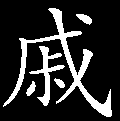
\includegraphics[width=3mm]{../Images/00005}总评:苏堤柳暖,阆苑春浓,兼之晨妆初罢,疏雨梧桐,正可借软草以慰佳人,采奇花以寄公子。不意莺嗔燕怒,逗起波涛,婆子长舌,丫鬟碎语,群相聚讼,又是一样烘云托月法。}

% {\href{../Text/part0063_split_000.html\#navto_1_a}{①}原作``杏叶渚'',除戚、列本作``柳叶渚'',他本均同底本。按``杏''字疑为``荇(莕)''之讹,此地实为前文已多次出现的``荇叶渚''。但诸本回目均作``柳叶渚'',为避免顾此失彼,仍依戚、列本改。}

% {\href{../Text/part0063_split_000.html\#navto_2_a}{②}``许多的不好的毛病'',除列本无``不好的''三字,它本均略同于底本。按``毛病''当然没有``好的'',列本删后似更合理,但口语多有不甚合乎逻辑者,现在也仍有``坏毛病''的说法,故不校改。}

% {\href{../Text/part0063_split_000.html\#navto_3_a}{③}``又有些较过'',戚、列本作``也省些交过''。据《汉语方言大词典》,``较过''为冀鲁官话,``日常开支''之意。今之新校本则多改为其他音近字。}
